\documentclass[8pt]{beamer}
% choosing beamer class
% \usepackage{beamerthemesplit} // Activate for custom appearance
\usepackage{graphics,amsmath, subfigure}
\usepackage[utf8]{inputenc} % as usual
\usetheme{Copenhagen}
\usefonttheme[?options ?]{structuresmallcapsserif}
\setbeamertemplate{caption}[numbered]


\title{Professional and Academic Experience} %Monday morning base class
\author{Hugo Day} %That'd be me
\date{28th January 2013}

\begin{document}

\frame{\titlepage}


\frame{
\frametitle{Contents}
\tableofcontents
}

\section{Education}
\frame{
\frametitle{Education}
\begin{itemize}
\item{PhD in Accelerator Physics, \textbf{University of Manchester}, Manchester, UK}
\begin{itemize}
\item{September 2009 - Present (Defence expected March 2013)}
\item{"Measurements and Simulations of Impedance Reduction Techniques in Particle Accelerators", under the supervision of Dr. Elias Métral (CERN) and Dr. Roger Jones (University of Manchester, UK).}
\end{itemize}
\item{MPhys Physics, \textbf{University of Southampton}, Southampton, UK}
\begin{itemize}
\item{October 2005 - July 2009. Grade: 1st Class}
\item{Supervisor - Dr. Malcolm Coe}
\item{Masters thesis "Controlling the Synthesis of Branched Gold Nanoparticles using a Wet Chemical Synthesis Method" under the supervision of Dr. Antonios Kanaras. Resulted in a journal paper in Crystal Engineering Communications Day, H.A., Bartczak, D., Fairbairn, N., Ardakani, M., Porter, A.E., Kanaras A. G. “Controlling the three-dimensional morphology of nanocrystals” CrystEngComm, 2010, 12, 4312-4316 doi:10.1039/C0CE00264J }
\end{itemize}
\end{itemize}
}

\section{Research}
\frame{
\frametitle{Research History}
\begin{itemize}
\item{During doctoral studies received a doctoral studentship from CERN, Switzerland. Spent 3 years (Feb 2010 - Jan 2013) on placement in the BE-ABP-ICE section at CERN. Under the supervision of Dr. Elias Metral, advised by Dr. Mike Barnes and Dr. Fritz Caspers.}
\item{Work focused on analysing the beam coupling impedance of two pieces of equipment in the LHC (injection kicker magnets (MKIs) and collimators) using 3D EM simulation programmes, such as CST Particle Studio and HFSS, and bench top measurements using the coaxial wire method. This was done in the context of beam-induced heating observed in the LHC during running of the LHC 2010-2012.}
\item{Work was completed in collaboration with the TE/ABT (MKIs) and EM/MME (Collimators) within in the ICE section working with a mixture of physicists, applied physicists, engineers and technicians of mixed nationalities and languages. Regular updates of the respective projects was given during meetings to specialised and general audiences, and the results presented at international conferences.}
\item{Gathered extensive experience working with computational EM solvers and CAD tools (Ansoft HFSS, CST:MWS), using python/matlab as an analysis tool. Extensive experience using RF measurement techniques, especially the use of VNAs and VSAs.}
\end{itemize}
}

\subsection{Doctoral Studies}
\frame{
\frametitle{LHC Injection Kicker Magnets}
\begin{itemize}
\item{MKIs had been measured to have very high temperatures during 2011/2012 (see Métral, Cham2012), requiring long cool down times ($\approx$2-3hrs) between fills - they proved to be a severe bottleneck for the availability of physics fills in the LHC.}
\item{A new beam screen was designed to reduce power loss in the structure, whilst avoiding excessive surface breakdown and increasing thermal radiation to the vacuum tank. This design will replace all magnets during LS1.}
\end{itemize}
\begin{figure}
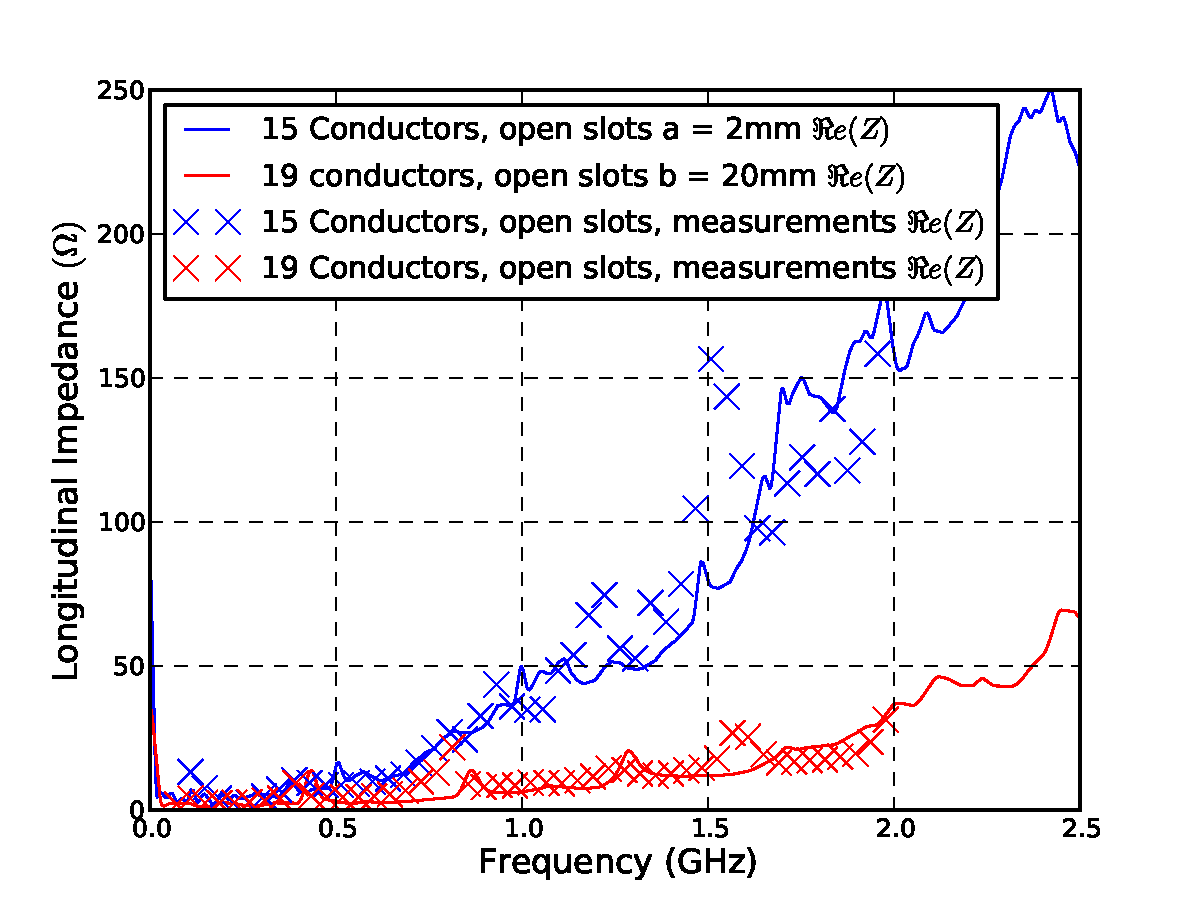
\includegraphics[width=0.5\textwidth]{15_19_sims_measured_comparison.pdf}
\caption{Comparison between simulations and coaxial wire measurements of the LHC injection kicker magnets.}
\end{figure}
WEPPR071, IPAC'12, New Orleans, US, 2012; MOPS078, IPAC'11, San Sebastian, Spain, 2011
}
\frame{
\begin{figure}
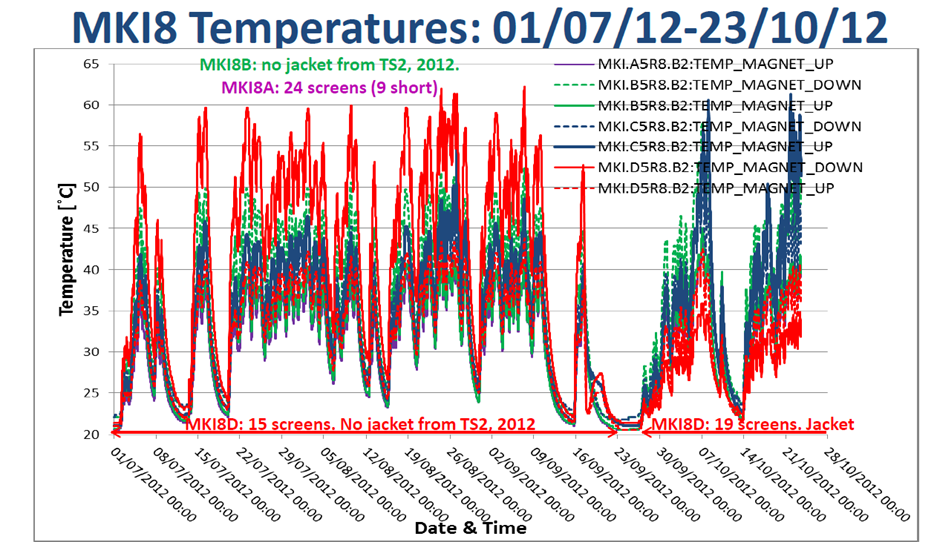
\includegraphics[width=0.95\textwidth]{mki8-temps-post-ts3.png}
\caption{The measured temperature of the MKIs before and after technical stop 3. MKI8d (red plot) had its beam screen modified during the technical stop, and it's measured temperature dropped significantly.}
\end{figure}
}

% Publications in the relevant areas of education or research
\frame{
\frametitle{Coaxial Wire Measurements}
\begin{itemize}
\item{Developments were made to the coaxial wire technique for measuring beam impedance to allow the measurement of the quadrupolar and constant transverse impedance terms of asymmetric structures and verified using computational simulations of analytical structures. Measurements of the MKI agree well also.}
\end{itemize}
\begin{figure}
\subfigure[]{
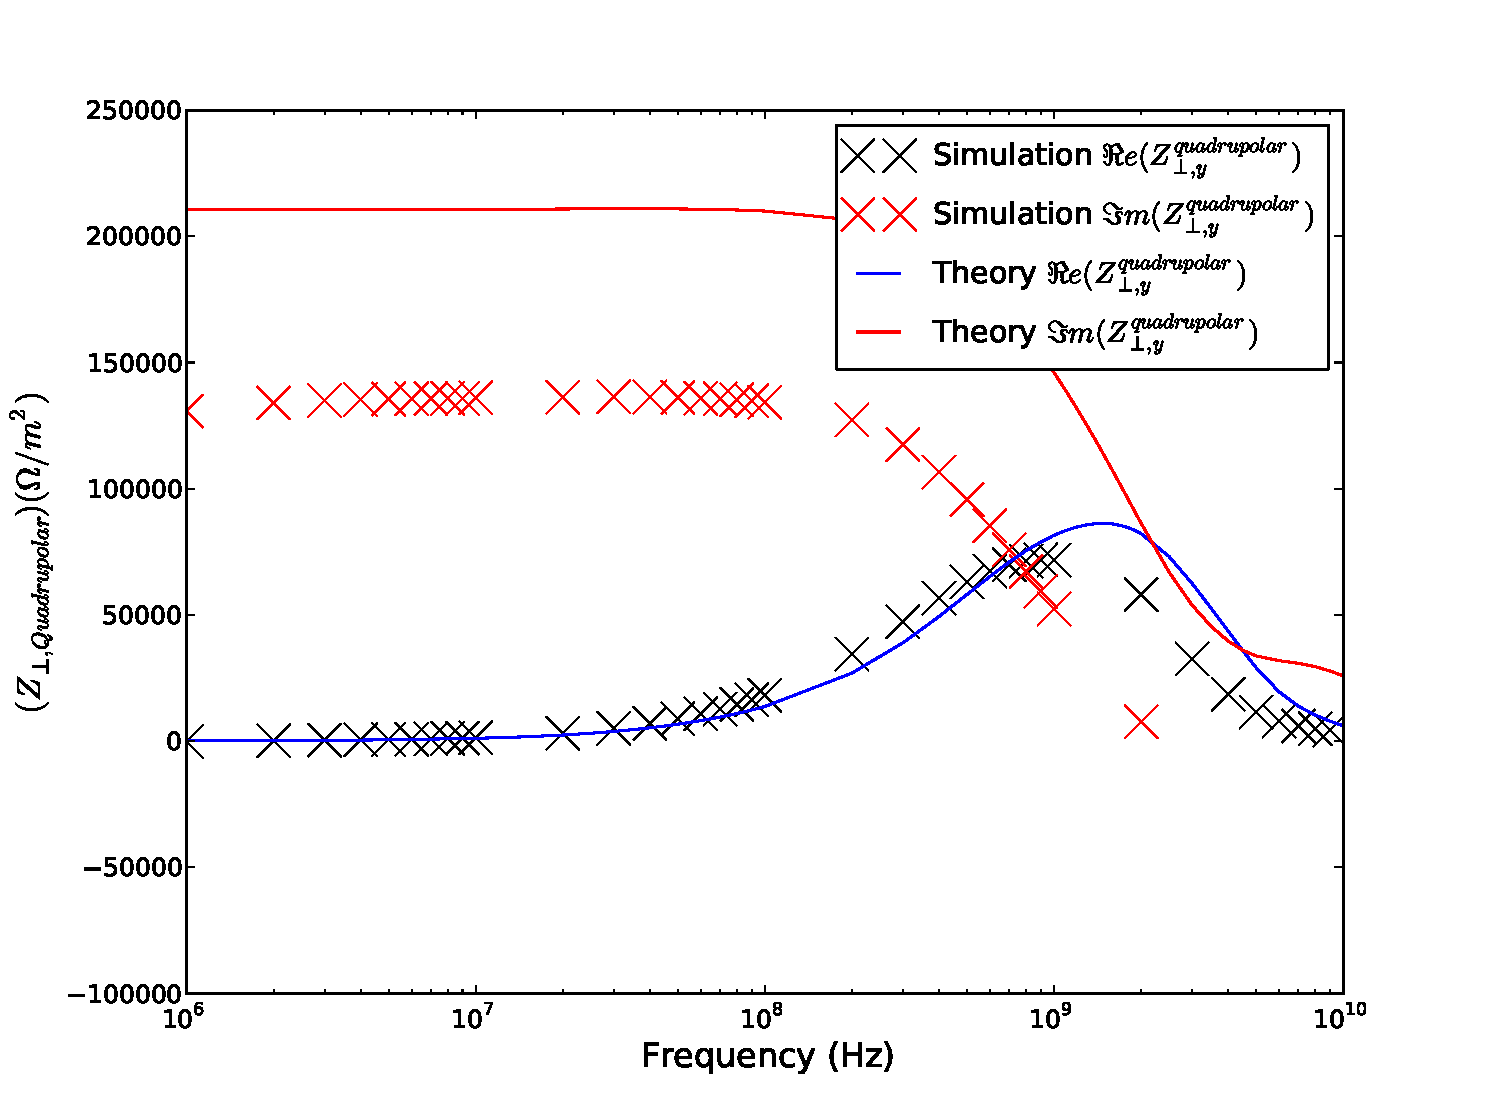
\includegraphics[width=0.45\textwidth]{quadrupolar-vertical-impedance.pdf}
\label{fig:quad-asym}
}
\subfigure[]{
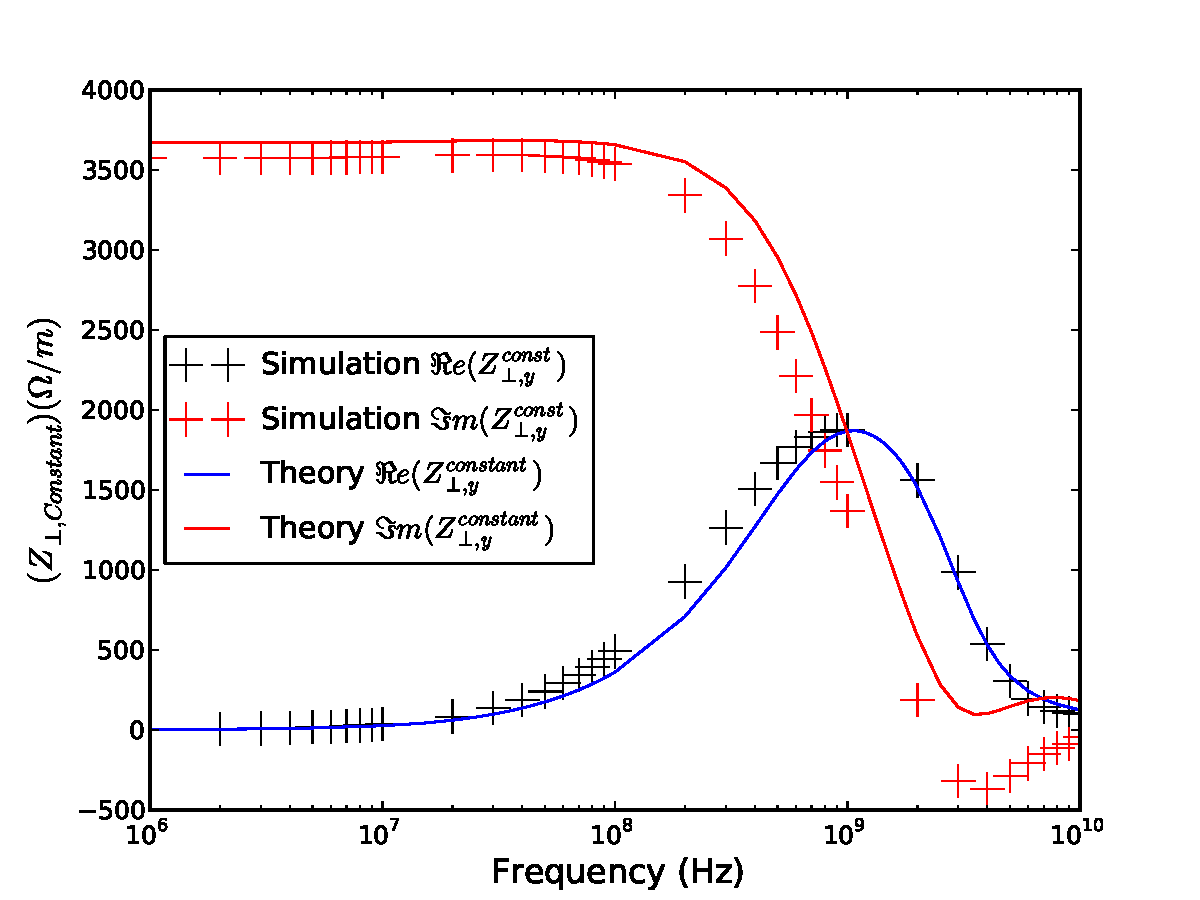
\includegraphics[width=0.45\textwidth]{constant-vertical-impedance.pdf}
\label{fig:const-asym}
}
\caption{Simulated coaxial wire measurements of an asymmetric device of the \ref{fig:quad-asym} quadrupolar and \ref{fig:const-asym} constant transverse impedances.}
\end{figure}
MOPS079, IPAC'11, San Sebastian, Spain, 2011
}

\frame{
\frametitle{Collimator RF System}
\begin{itemize}
\item{A new impedance reduction scheme for the LHC collimators was evaluated in the context of the newly designed TCTP collimator for the LHC. This contactless design used a system of damping ferrites to de-Q cavity modes in the tank, as the older system was a suspected cause of dust particles in the LHC. In this context a rigourous study of the location of the power loss in ferrite damped structures from weak to strong damping was done to see how the amount of damping changed the power loss to the ferrites.}
\end{itemize}
WEPPR070, IPAC'12, New Orleans, US, 2012; MOPS080, IPAC'11, San Sebastian, Spain, 2011 
}

\subsection{Nanotechnology}
\frame{
\frametitle{Nanotechnology}
\begin{itemize}
\item{Masters project involved working with the Laboratory for Inorganic Colloidal Nanocrystals, Southampton University on the subject of controlling the morphological structure of branched gold nanoparticles by variation of a known synthesis method. Gained a deal of experience of laboratory working practices and experimental practice.}
\item{Significant progress was made in understanding the reaction mechanisms, and subsequently controlling morphological factors such as branch size, number of branches and core size.}
\end{itemize}
\begin{figure}
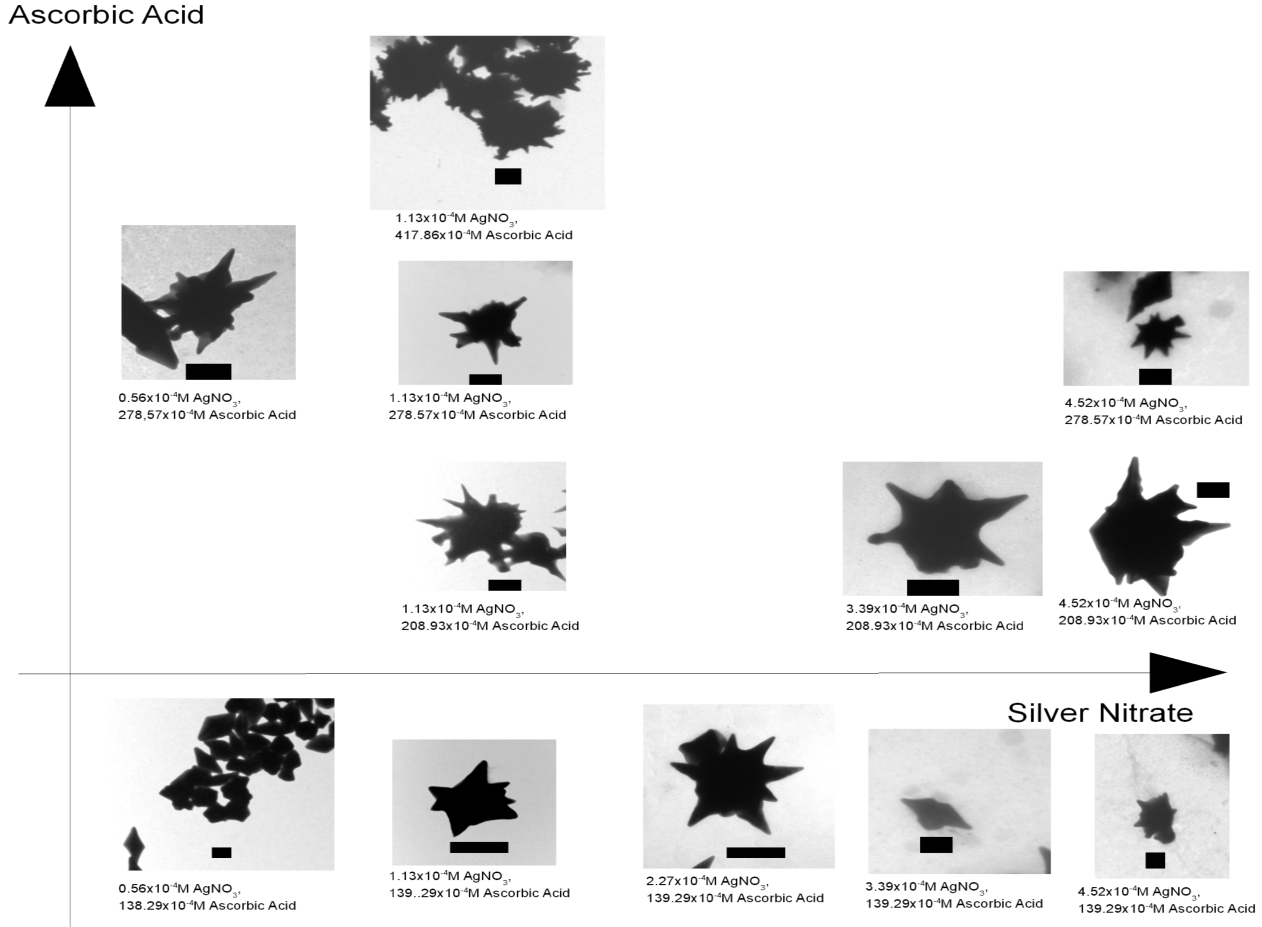
\includegraphics[width=0.45\textwidth]{nanoParticles.png}
\end{figure}
}

\frame{
\frametitle{Thanks for listening, any questions?}
}


\end{document}
